% Source: Lecture8a.pdf, pages 1-4 (page 1 is a title page; page 5 is blank). Title on the source:
% "Lecture 8a (to be used in conjunction with the printed slides in Lecture 8)".
\lecture{8a}
\subsection{Further notes for Lecture 8: examples of graphs}

These notes are to be used in conjunction with the printed slides of Lecture 8.

\tikzset{gv/.style={circle,fill,inner sep=0pt,minimum size=4pt}}

\begin{diagram}
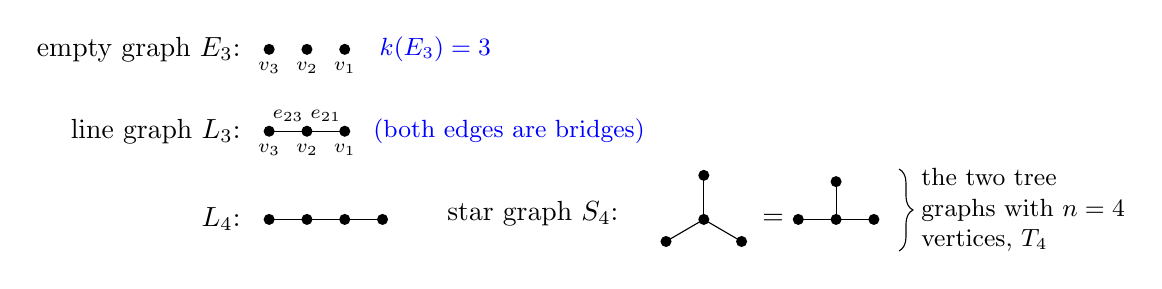
\begin{tikzpicture}[scale=0.8]
  \node[anchor=east] at (-0.3,0) {empty graph $E_3$:};
  \foreach \x/\l in {0/v_3,0.6/v_2,1.2/v_1} {\node[gv] at (\x,0) {}; \node[below,font=\scriptsize] at (\x,-0.05) {$\l$};}
  \node[blue,anchor=west,font=\small] at (1.6,0) {$k(E_3) = 3$};
  \begin{scope}[yshift=-1.3cm]
    \node[anchor=east] at (-0.3,0) {line graph $L_3$:};
    \draw (0,0) -- (1.2,0);
    \foreach \x/\l in {0/v_3,0.6/v_2,1.2/v_1} {\node[gv] at (\x,0) {}; \node[below,font=\scriptsize] at (\x,-0.05) {$\l$};}
    \node[above,font=\scriptsize] at (0.3,0) {$e_{23}$}; \node[above,font=\scriptsize] at (0.9,0) {$e_{21}$};
    \node[blue,anchor=west,font=\small] at (1.5,0) {(both edges are bridges)};
  \end{scope}
  \begin{scope}[yshift=-2.7cm]
    \node[anchor=east] at (-0.3,0) {$L_4$:};
    \draw (0,0) -- (1.8,0); \foreach \x in {0,0.6,1.2,1.8} \node[gv] at (\x,0) {};
    \begin{scope}[xshift=1.2cm]
    \node[anchor=east] at (4.5,0.1) {star graph $S_4$:};
    \draw (5.7,0) -- (5.7,0.7); \draw (5.7,0) -- (5.1,-0.35); \draw (5.7,0) -- (6.3,-0.35);
    \foreach \p in {(5.7,0),(5.7,0.7),(5.1,-0.35),(6.3,-0.35)} \node[gv] at \p {};
    \node at (6.8,0) {$=$};
    \draw (7.2,0) -- (8.4,0); \draw (7.8,0) -- (7.8,0.6);
    \foreach \p in {(7.2,0),(7.8,0),(8.4,0),(7.8,0.6)} \node[gv] at \p {};
    \draw[decorate,decoration={brace,amplitude=5pt}] (8.8,0.8) -- (8.8,-0.5);
    \node[anchor=west,font=\small,align=left] at (9.0,0.15) {the two tree\\ graphs with $n = 4$\\ vertices, $T_4$};
    \end{scope}
  \end{scope}
\end{tikzpicture}
\diagramcaption{Some types of graphs.}
\end{diagram}

\begin{diagram}
\begin{tikzpicture}[scale=0.8]
  % circuit graphs
  \node[gv] (a) at (0,0) {}; \draw (0,0) .. controls (-0.5,0.9) and (0.5,0.9) .. (0,0);
  \node[below] at (0,-0.4) {$C_1$}; \node[blue,font=\scriptsize] at (-0.6,0.8) {loop};
  \draw (1.6,0.25) circle (0.45); \node[gv] at (1.15,0.25) {}; \node[gv] at (2.05,0.25) {}; \node[below] at (1.6,-0.4) {$C_2$};
  \draw (3.4,0.25) circle (0.45); \foreach \a in {90,210,330} \node[gv] at ($(3.4,0.25)+(\a:0.45)$) {}; \node[below] at (3.4,-0.4) {$C_3$};
  \draw (5.2,0.25) circle (0.45); \foreach \a in {45,135,225,315} \node[gv] at ($(5.2,0.25)+(\a:0.45)$) {};
  \node at (6.0,0.25) {$=$}; \draw (6.4,-0.1) rectangle (7.1,0.6);
  \foreach \p in {(6.4,-0.1),(7.1,-0.1),(6.4,0.6),(7.1,0.6)} \node[gv] at \p {};
  \node[below] at (5.8,-0.4) {$C_4$};
  \node at (3.5,1.3) {circuit graphs};
  % complete graphs
  \begin{scope}[xshift=8.6cm]
    \node at (2.4,1.3) {complete graphs};
    \draw (0,0.25) -- (0.8,0.25); \node[gv] at (0,0.25) {}; \node[gv] at (0.8,0.25) {};
    \node[below] at (0.4,-0.4) {$K_2 = L_2$};
    \draw (2.0,-0.1) -- (2.8,-0.1) -- (2.4,0.6) -- cycle;
    \foreach \p in {(2.0,-0.1),(2.8,-0.1),(2.4,0.6)} \node[gv] at \p {};
    \node[below] at (2.4,-0.4) {$K_3 = C_3$};
    \coordinate (A) at (3.8,-0.1); \coordinate (B) at (4.8,-0.1); \coordinate (Cc) at (4.3,0.75); \coordinate (D) at (4.3,0.2);
    \draw (A) -- (B) -- (Cc) -- cycle; \draw (A) -- (D) -- (B); \draw (Cc) -- (D);
    \foreach \p in {A,B,Cc,D} \node[gv] at (\p) {};
    \node[below] at (4.3,-0.4) {$K_4$};
  \end{scope}
\end{tikzpicture}
\diagramcaption{Circuit graphs $C_n$ and complete graphs $K_n$.}
\end{diagram}

\paragraph{Cycles in a graph.} For the square with one diagonal,
\begin{equation}
  c(G) = e(G)+k(G)-n(G) = 5+1-4 = 2 .
\end{equation}
There are 3 cycles, but only 2 are linearly independent; by combining the inner two cycles, one obtains the outer cycle.

\begin{diagram}
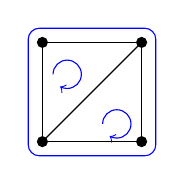
\begin{tikzpicture}[scale=0.9]
  \draw (0,0) rectangle (1.4,1.4); \draw (0,0) -- (1.4,1.4);
  \foreach \p in {(0,0),(1.4,0),(0,1.4),(1.4,1.4)} \node[gv] at \p {};
  \draw[blue,->] (0.15,0.95) arc (180:-120:0.2);
  \draw[blue,->] (0.85,0.25) arc (180:-120:0.2);
  \draw[blue,->,rounded corners] (-0.2,-0.2) rectangle (1.6,1.6);
\end{tikzpicture}
\diagramcaption{The square with a diagonal edge: two independent inner cycles and the outer cycle.}
\end{diagram}

\subsection{Spanning subgraphs and the Tutte polynomial of \texorpdfstring{$C_3$}{C3}}

Spanning subgraphs (SSG): e.g.\ let $G = C_3 = K_3$; $G = (V,E)$; $G' = (V,E')$, $E'\subseteq E$. The spanning subgraphs
$\{G'\}$ are:

\begin{diagram}
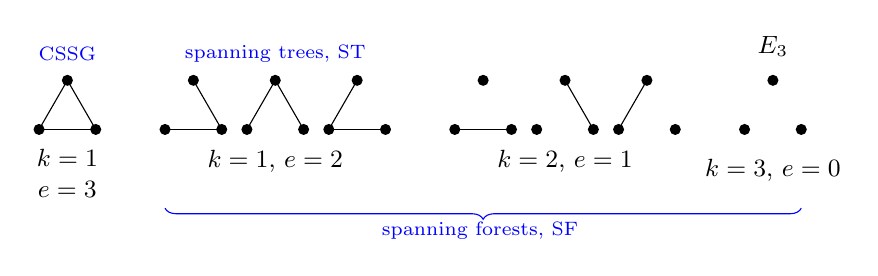
\begin{tikzpicture}[scale=0.8]
  \newcommand{\tri}[4]{%
    \begin{scope}[xshift=#1 cm]
      \coordinate (P1) at (0,0); \coordinate (P2) at (0.9,0); \coordinate (P3) at (0.45,0.78);
      \foreach \p in {P1,P2,P3} \node[gv] at (\p) {};
      \ifnum#2=1 \draw (P1) -- (P2);\fi
      \ifnum#3=1 \draw (P2) -- (P3);\fi
      \ifnum#4=1 \draw (P3) -- (P1);\fi
    \end{scope}}
  \tri{0}{1}{1}{1}
  \node[font=\small,align=center] at (0.45,-0.7) {$k = 1$\\ $e = 3$};
  \tri{2.0}{1}{1}{0} \tri{3.3}{0}{1}{1} \tri{4.6}{1}{0}{1}
  \node[font=\small] at (3.75,-0.5) {$k = 1$, $e = 2$};
  \tri{6.6}{1}{0}{0} \tri{7.9}{0}{1}{0} \tri{9.2}{0}{0}{1}
  \node[font=\small] at (8.35,-0.5) {$k = 2$, $e = 1$};
  \tri{11.2}{0}{0}{0}
  \node[font=\small,align=center] at (11.65,-0.65) {$k = 3$, $e = 0$};
  \node[font=\small,anchor=south] at (11.65,1.0) {$E_3$};
  \node[blue,font=\scriptsize] at (0.45,1.2) {CSSG};
  \node[blue,font=\scriptsize] at (3.75,1.2) {spanning trees, ST};
  \draw[blue,decorate,decoration={brace,amplitude=4pt,mirror}] (2.0,-1.25) -- (12.1,-1.25);
  \node[blue,font=\scriptsize] at (7.0,-1.6) {spanning forests, SF};
\end{tikzpicture}
\diagramcaption{The $2^3 = 8$ spanning subgraphs of $C_3$. CSSG = connected spanning subgraphs. Note: one of the $G'$ is $G$
itself.}
\end{diagram}

From $T(C_n,x,y) = \left[\sum_{j=1}^{n-1}x^j\right]+y$,
\begin{equation}
  T(C_3,x,y) = x+x^2+y,
\end{equation}
and
\begin{align}
  T(C_3,1,1) &= N_{ST}(C_3) = 3, & T(C_3,1,2) &= N_{CSSG}(C_3) = 4,\\
  T(C_3,2,1) &= N_{SF}(C_3) = 7, & T(C_3,2,2) &= N_{SSG}(C_3) = 8 .
\end{align}

\subsection{\texorpdfstring{$k$}{k}-partite graphs}

$k$-partite graphs: $G = G(V,E)$ such that $V = V_1\cup V_2\cup\cdots\cup V_k$, where $\{V_i\}$ are subsets of $V$, such that no
edge connects a vertex in $V_i$ to another vertex in $V_i$. Any loopless $n$-vertex graph is $n$-partite with $V_i = \{v_i\}$.
Examples of bipartite graphs: the line graph $L_n$ for any $n$; the circuit graph $C_n$ if $n$ is even, but not $C_n$, $n$ odd.
Tripartite examples: $L_3$ (colored with three colors) and the triangular lattice with free boundary conditions (FBC).

\begin{diagram}
\begin{tikzpicture}[scale=0.8]
  \draw (0,0) -- (0.8,0); \fill[red] (0,0) circle (0.09); \fill[blue] (0.8,0) circle (0.09); \node[below] at (0.4,-0.2) {$L_2$};
  \draw (1.6,0) -- (3.2,0); \fill[red] (1.6,0) circle (0.09); \fill[blue] (2.4,0) circle (0.09); \fill[red] (3.2,0) circle (0.09);
  \node[below] at (2.4,-0.2) {$L_3$};
  \draw (4.6,0) circle (0.5);
  \fill[blue] (4.6,0.5) circle (0.09); \fill[red] (5.1,0) circle (0.09); \fill[blue] (4.6,-0.5) circle (0.09); \fill[red] (4.1,0) circle (0.09);
  \node[below] at (4.6,-0.55) {$C_4$};
  \draw (7.0,0) circle (0.5);
  \fill[blue] (7.0,0.5) circle (0.09); \fill[red] ($(7.0,0)+(210:0.5)$) circle (0.09); \fill[blue] ($(7.0,0)+(330:0.5)$) circle (0.09);
  \node[below,align=center] at (7.0,-0.55) {$C_3$\\ (not bipartite)};
  \begin{scope}[xshift=10.0cm,yshift=0cm,scale=0.8]
    \draw (0,0) -- (1.6,0); \fill[red] (0,0) circle (0.11); \fill[green!60!black] (0.8,0) circle (0.11); \fill[blue] (1.6,0) circle (0.11);
    \node[below,align=center] at (0.8,-0.25) {$L_3$,\\ tripartite};
  \end{scope}
\end{tikzpicture}
\diagramcaption{Bipartite graphs $L_2$, $L_3$, $C_4$; the odd circuit $C_3$ is not bipartite. Right: a 3-coloring of $L_3$.}
\end{diagram}

For a line graph (or any tree), $P(L_n,q) = P(T_n,q) = q(q-1)^{n-1}$, and for a triangular lattice with FBC,
$P(\text{tri lattice, FBC},q=3) = 3!$, as in the coloring of Figure~\ref{fig:tri3col}.

\begin{diagram}
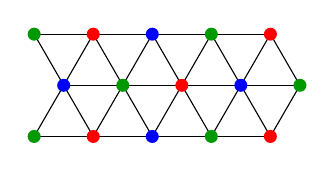
\begin{tikzpicture}[scale=0.75]
  \foreach \j in {0,1,2} \draw ({0.5*mod(\j,2)},{0.866*\j}) -- ++(4,0);
  \foreach \i in {0,...,4} {\draw (\i,0) -- ++(60:1) -- ++(120:1);}
  \foreach \i in {1,...,4} {\draw (\i,0) -- ++(120:1) -- ++(60:1);}
  \foreach \j in {0,1,2} \foreach \i in {0,...,4} {
    \pgfmathtruncatemacro{\c}{mod(\i-floor(\j/2)-\j+30,3)}
    \pgfmathsetmacro{\xx}{\i+0.5*mod(\j,2)}
    \ifnum\c=0 \fill[green!60!black] (\xx,{0.866*\j}) circle (0.11);\fi
    \ifnum\c=1 \fill[red] (\xx,{0.866*\j}) circle (0.11);\fi
    \ifnum\c=2 \fill[blue] (\xx,{0.866*\j}) circle (0.11);\fi
  }
\end{tikzpicture}
\diagramcaption{A proper 3-coloring of a section of the triangular lattice with free boundary conditions.}\label{fig:tri3col}
\end{diagram}

\subsection{Planar duality}

E.g.\ let $G = C_3 = K_3$. The triangle has two faces, the interior and the exterior, so its dual has two vertices, joined by one
edge for each of the three edges of the triangle: $C_3^*$ is the ``fat link'' $FL_3$, where $FL_n$ denotes two vertices joined by
$n$ edges.

\begin{diagram}
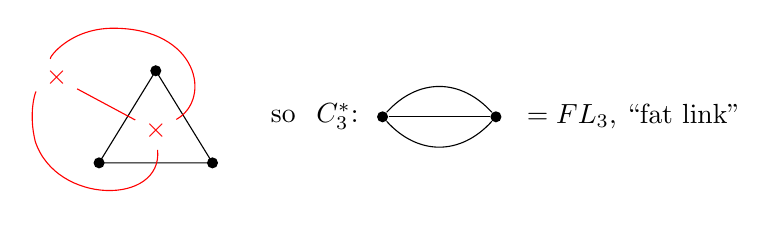
\begin{tikzpicture}[scale=0.9]
  \coordinate (A) at (0,0); \coordinate (B) at (1.6,0); \coordinate (Cc) at (0.8,1.3);
  \draw (A) -- (B) -- (Cc) -- cycle; \foreach \p in {A,B,Cc} \node[gv] at (\p) {};
  \node[red] (in) at (0.8,0.45) {$\times$}; \node[red] (out) at (-0.6,1.2) {$\times$};
  \draw[red] (in) -- (out);
  \draw[red] (in) .. controls (1.6,0.9) and (1.4,1.9) .. (0.2,1.9) .. controls (-0.4,1.9) and (-0.7,1.5) .. (out);
  \draw[red] (in) .. controls (0.9,-0.6) and (-0.6,-0.6) .. (-0.9,0.3) .. controls (-1.0,0.7) and (-0.9,1.0) .. (out);
  \node at (2.6,0.65) {so};
  \begin{scope}[xshift=4cm,yshift=0.65cm]
    \node[anchor=east] at (-0.2,0) {$C_3^*$:};
    \node[gv] (p) at (0,0) {}; \node[gv] (q) at (1.6,0) {};
    \draw (p) -- (q); \draw (p) .. controls (0.5,0.55) and (1.1,0.55) .. (q); \draw (p) .. controls (0.5,-0.55) and (1.1,-0.55) .. (q);
    \node[anchor=west] at (1.9,0) {$= FL_3$, ``fat link''};
  \end{scope}
\end{tikzpicture}
\diagramcaption{The planar dual of the triangle $C_3$: one dual vertex ($\times$) inside the triangle and one outside, joined by
three edges.}
\end{diagram}

A lattice example: $(\Lambda_{tri})^* = \Lambda_{hc}$, where tri = triangular lattice and hc = honeycomb lattice. The faces of the
triangular lattice become the vertices of the honeycomb lattice (see Figure~\ref{fig:duality}, read from right to left).

\subsection{The deletion--contraction relation}

DCR = deletion--contraction relation for the chromatic polynomial ($T = 0$ Potts antiferromagnet): consider a graph $G$ and an
edge $e$ in $G$; then
\begin{equation}
  P(G,q) = P(G-e,q) - P(G/e,q),
\end{equation}
where $G-e$ is the graph with $e$ deleted and $G/e$ is the graph with $e$ deleted and the vertices that had been connected via
$e$ contracted (to become a single vertex).

\paragraph{Proof.} We will prove the equivalent relation
\begin{equation}
  P(G-e,q) = P(G,q) + P(G/e,q).
\end{equation}
Consider the proper $q$-colorings of $G-e$. These consist of two classes: (i) colorings with $q(v_i)\ne q(v_j)$, which are
enumerated by $P(G,q)$, since the edge $e$ enforces this condition, and (ii) colorings with $q(v_i) = q(v_j)$; these are
enumerated by $P(G/e,q)$, where we delete $e$ and identify $v_i = v_j$.

\begin{diagram}
\begin{tikzpicture}[scale=0.9]
  \newcommand{\blob}[1]{\draw[pattern=north east lines] (#1) ellipse (0.45 and 0.25);}
  \blob{0,0} \node[gv] (a) at (-0.25,0.7) {}; \node[gv] (b) at (0.25,0.7) {};
  \draw (a) -- (-0.2,0.2); \draw (b) -- (0.2,0.2);
  \node[left,font=\scriptsize] at (-0.25,0.75) {$v_i$}; \node[right,font=\scriptsize] at (0.25,0.75) {$v_j$};
  \node[font=\small] at (0,-0.6) {$G-e$};
  \begin{scope}[xshift=3cm]
    \blob{0,0} \node[gv] (a) at (-0.25,0.7) {}; \node[gv] (b) at (0.25,0.7) {};
    \draw (a) -- (-0.2,0.2); \draw (b) -- (0.2,0.2); \draw (a) -- node[above,font=\scriptsize] {$e$} (b);
    \node[left,font=\scriptsize] at (-0.25,0.75) {$v_i$}; \node[right,font=\scriptsize] at (0.25,0.75) {$v_j$};
    \node[font=\small] at (0,-0.6) {$G$};
  \end{scope}
  \begin{scope}[xshift=6cm]
    \blob{0,0} \node[gv] (a) at (0,0.75) {}; \draw (a) -- (-0.2,0.2); \draw (a) -- (0.2,0.2);
    \node[right,font=\scriptsize] at (0.05,0.8) {$v_i = v_j$};
    \node[font=\small] at (0,-0.6) {$G/e$};
  \end{scope}
\end{tikzpicture}
\diagramcaption{The graphs $G-e$, $G$ and $G/e$ near the edge $e$; the shaded region is the rest of the graph.}
\end{diagram}

E.g.\ for the single edge $K_2$:
\begin{equation}
  P(K_2,q) = P(E_2,q) - P(E_1,q):\qquad q(q-1) = q^2-q .
\end{equation}

N.B.: the chromatic polynomial of a graph in which two vertices are connected by more than one edge is the same as the chromatic
polynomial where they are connected by a single edge. For example, $P(C_2,q) = P(K_2,q)$.

Another example: apply the DCR to one edge of the triangle (marking the edge that is deleted):
\begin{equation}
  P(K_3,q) = P(L_3,q) - P(C_2,q),\qquad
  q(q-1)(q-2):\quad q(q-1)^2 - q(q-1) = q(q-1)(q-2),
\end{equation}
using $P(C_2,q) = P(K_2,q) = q(q-1)$.
